\documentclass[tikz,border=10pt]{standalone}
\begin{document}
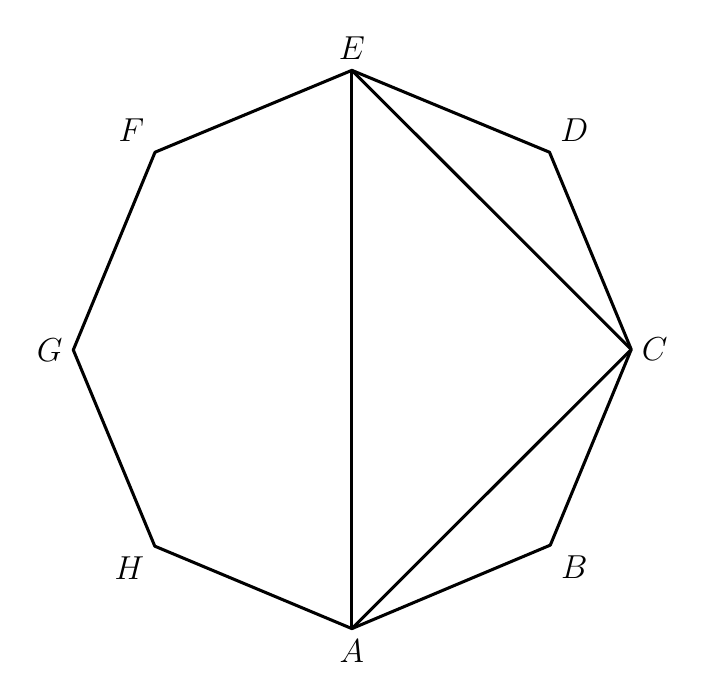
\begin{tikzpicture}[line join=round, line width=1.1pt]
\coordinate (A) at (-0.010,-3.540);
\coordinate (B) at (2.510,-2.480);
\coordinate (C) at (3.538,0.005);
\coordinate (D) at (2.500,2.510);
\coordinate (E) at (-0.010,3.550);
\coordinate (F) at (-2.510,2.510);
\coordinate (G) at (-3.548,-0.001);
\coordinate (H) at (-2.513,-2.493);

  
  \draw (A) -- (B) -- (C) -- (D) -- (E) -- (F) -- (G) -- (H) -- cycle;
  
  \draw (A) -- (E);
  \draw (E) -- (C);
  \draw (C) -- (A);
  
  \node[above] at (E) {\fontsize{11.5}{13.8}\selectfont $E$};
  \node[above right] at (D) {\fontsize{11.5}{13.8}\selectfont $D$};
  \node[right] at (C) {\fontsize{11.5}{13.8}\selectfont $C$};
  \node[below right] at (B) {\fontsize{11.5}{13.8}\selectfont $B$};
  \node[below] at (A) {\fontsize{11.5}{13.8}\selectfont $A$};
  \node[below left] at (H) {\fontsize{11.5}{13.8}\selectfont $H$};
  \node[left] at (G) {\fontsize{11.5}{13.8}\selectfont $G$};
  \node[above left] at (F) {\fontsize{11.5}{13.8}\selectfont $F$};
\end{tikzpicture}
\end{document}